\documentclass{article}

% Packages
\usepackage{graphicx} % For including images
\usepackage{amsmath} % For mathematical symbols and equations
\usepackage{cite} % For citing references
\usepackage{hyperref} % For hyperlinks

% Title
\title{%
  Let's Beat Geometry Dash \\
  \large APS350 Project Proposal
  }
\author{JV, IL, SH, JD}
\date{\today}

\begin{document}

\maketitle

\pagebreak
\section{Introduction (4 marks)}
Geometry Dash is a popular platformer video game 
where the player attempts to navigate through 
obstacles in order to reach the end of a level. 
The game features a variety of game modes and 
unique objects.

A video of the first level can be seen \href{https://www.youtube.com/watch?v=bbVEbqU9wPo}{here:} 

\begin{center} 
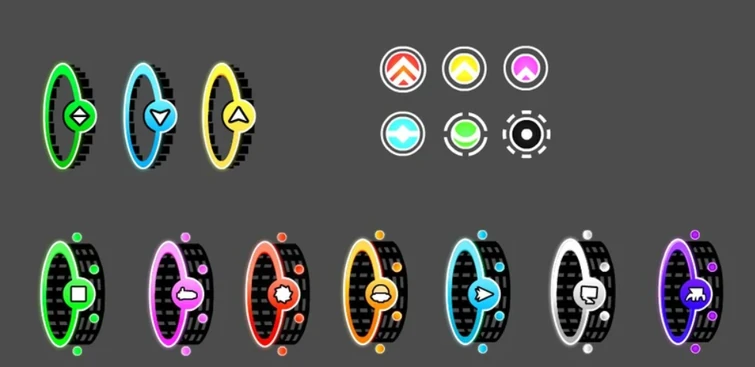
\includegraphics[scale=0.5]{Images/GeoObj.png}
\end{center}




\section{Background and Related Work (4 marks)}
% Your methods here

\section{Data Processing (2 marks)}
% Your methods here

\section{Architecture (2 marks)}
% Your results here

\section{Baseline Model (2 marks)}
% Your discussion here

\section{Ethical Considerations (2 marks)}
Geometry Dash has online levels that users can play to earn rewards 
such as diamonds, orbs, and stars. These stars can be used to rank 
the player on the global leaderboard. Developing a bot that can complete 
Geometry Dash with machine learning can result in players gaining an 
unfair advantage over their peers as they climb the leaderboard, and 
result in people playing the game in a way the developers did not intend.

Another ethical consideration could be in the training of the models. 
It is unethical to use the work of others for profit without their 
permission. Levels that are created and published by Geometry Dash 
users online are their own creative works, and it may be unethical to 
use their work to train a model that can be used to generate an income 
without their consent. As a result, our group does not intend to 
commercialize this project.


\section{Project Plan (4 marks)}
% Your conclusion here

\section{Risk Registrar (4 marks)}
The largest potential risk of this project is that we are unable to 
finish. We would like to train a bot that can complete Geometry Dash, 
but this would require that we finish training both the CNN model and 
the RL model in time. If we are unable to finish both, our group would 
just submit the CNN model for our final submission, as the CNN model 
would fulfill the requirements of this project, while the RL model is 
beyond the scope of this course. Although an RL model would be nice, 
we may have to sacrifice it if time does not permit. 

There is also a risk that our group will not even finish the CNN model 
in time. There is a risk that our group will leave deliverables to the 
last minute, resulting in too little time to properly train our model 
and embark on the iterative process of trial and failure that marks all
successful projects. To combat this tendency, we have decided as a team 
to implement many internal deadlines so that our model will have plenty 
of time to train.

Another potential risk of this project could be that our code only works
on one machine, as the course instructor made it clear that the TA grading
our project should be able to run our code. We intend to make the bot 
able to play Geometry Dash, which could require that our bot access the 
keyboard on its host computer, which could involve different libraries 
and processes for different machines and operating systems. Although 
we could try to mitigate this as much as possible by testing on various 
computers and making sure it works on all of our different machines, time
constraints may disallow us from solving this issue in time. If we are 
unable to guarantee that it can run on any machine, we may have to preface 
our final submission with a warning that it only runs on a certain 
operating system. As of right now, our team plans to develop our model 
for Geometry Dash on Linux. 

Lastly, there is the risk that one of our team members is unable to finish
their portion of the project due to an outside situation. Fortunately, 
we have clearly outlined the responsibilities and tasks of each teammate, 
so if a teammate is unable to complete their tasks on time, it will be 
easy for the other teammates to recognize what still needs to be done.


\section{Github Link (1 Mark)}
https://github.com/J-Vadakken/APS360-Project

% References
\begin{thebibliography}{9}
\bibitem{reference1}
Author 1, Title of the paper, Journal name, Year.

\bibitem{reference2}
Author 2, Title of the paper, Conference name, Year.
\end{thebibliography}

\end{document}
